$\displaystyle \int_{-\infty}^{+\infty} \frac{dx}{1+4x^2}$

\nopagebreak
\begin{align*}
I &= \int_{-\infty}^{+\infty} \frac{dx}{1+(2x)^2} \\
\text{Sustitución: } u=2x, du=2dx \implies dx=du/2. \\
I &= \frac{1}{2} \int_{-\infty}^{+\infty} \frac{du}{1+u^2} \\
&= \frac{1}{2} [\arctan u]_{-\infty}^{+\infty} \\
&= \frac{1}{2} (\frac{\pi}{2} - (-\frac{\pi}{2})) = \frac{1}{2} (\pi) = \frac{\pi}{2}
\end{align*}

\[
\boxed{\displaystyle \frac{\pi}{2}}
\]

\begin{center}
    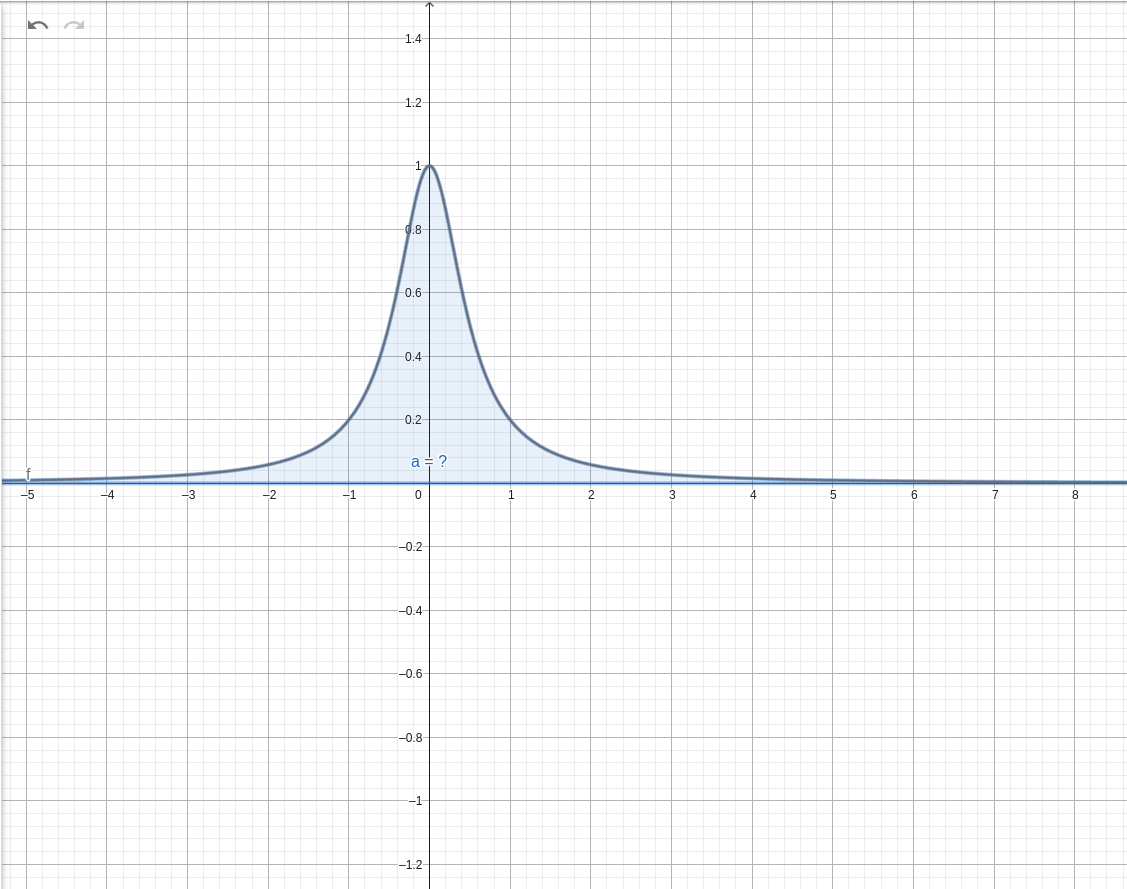
\includegraphics[width=0.5\textwidth]{Graficas/ejer44.png}
\end{center}
